% ****** Start of file aipsamp.tex ******
%
%   This file is part of the AIP files in the AIP distribution for REVTeX 4.
%   Version 4.1 of REVTeX, October 2009
%
%   Copyright (c) 2009 American Institute of Physics.

% Use this file as a source of example code for your aip document.
% Use the file aiptemplate.tex as a template for your document.
\documentclass[%
 aip,
 jmp,%
 amsmath,amssymb,
%preprint,%
 reprint,%
%author-year,%
%author-numerical,%
]{revtex4-1}

\usepackage{graphicx}% Include figure files
\usepackage{grffile}
\usepackage{dcolumn}% Align table columns on decimal point
\usepackage{bm}% bold math
%\usepackage[mathlines]{lineno}% Enable numbering of text and display math
%\linenumbers\relax % Commence numbering lines
\usepackage{hyperref}
\usepackage{multirow}
\usepackage{color} % for the notes
\usepackage{etex}
\reserveinserts{58}
\usepackage{morefloats}

\usepackage{longtable}
\usepackage{float}
\usepackage{supertabular}

\usepackage{booktabs}
\usepackage{array}
\usepackage{xr}
\externaldocument{supportingInformation}
\usepackage[section] {placeins}

 
%%%%%%%%%%%%
\usepackage{listings}
\usepackage{xcolor}       
\definecolor{dkgreen}{rgb}{0,0.6,0}
\definecolor{gray}{rgb}{0.5,0.5,0.5}
\definecolor{light-gray}{rgb}{0.97,0.97,0.97}

\lstdefinelanguage{owlms}
    {morekeywords={xsd,owl,xml,dc,rdf,skos,description,PlainLiteral,int,float,
        some,only,value,min,exactly,max,and,or,not,
        Prefix,Ontology,Import,Individual,Facts,Types,Class,
        DataProperty,ObjectProperty,AnnotationProperty,Annotations,
        DifferentIndividuals,SubClassOf,EquivalentTo,DisjointWith,DisjointUnionOf,SubPropertyOf,DisjointClasses,DisjointProperties,
        Symmetric,Asymmetric,Reflexive,Irreflexive,Transitive,Functional,InverseFunctional,
        Characteristics,Range,Domain,Datatype},
     basicstyle=\scriptsize\ttfamily,
     backgroundcolor=\color{light-gray},
     keywordstyle=\color{blue},
     commentstyle=\color{gray},
     stringstyle=\color{dkgreen},
     numbers=left,
     numberstyle=\tiny\color{gray},
     stepnumber=1,
     numbersep=10pt,
     tabsize=2,
     showspaces=false,
     showstringspaces=false,
     breaklines=true,                           % wrap text
     sensitive=true,                            % keywords are case sensitive
     morecomment=[l][commentstyle]{\#},         % comment format
     morestring=[b]",                           % string format
}

\hypersetup{
	colorlinks,
	linkcolor={red!50!black},
	citecolor={blue!50!black},
	urlcolor={blue!80!black}
}


\begin{document}

\preprint{XXXXX (preprint)}

%\title[Text differentiation in interaction networks]{A connective differentiation of text in interaction networks}% Force line breaks with \\
\title[Text and topology in interaction networks]{Text and topology in in human interaction networks: differences among Erd\"os sectors and correlation of metrics}% Force line breaks with \\

\author{Renato Fabbri}%
% \homepage{http://ifsc.usp.br/~fabbri/}
 \email{fabbri@usp.br}
  \affiliation{ 
Instituto de F\'isica de S\~ao Carlos, Universidade de S\~ao Paulo (IFSC/USP)%\\This line break forced with \textbackslash\textbackslash
}%
%\author{Vilson Vieira da Silva Junior}
%  \homepage{http://automata.cc/}
%  \email{vilson@void.cc}
%  \altaffiliation[Also at ]{IFSC-USP}%Lines break automatically or can be forced with \\
%
%\author{Ricardo Fabbri}
%  \homepage{http://www.lems.brown.edu/~rfabbri/}
%  \email{rfabbri@iprj.uerj.br}
% \altaffiliation{
%Instituto Polit\'ecnico, Universidade Estadual do Rio de Janeiro (IPRJ)
%}%Lines break automatically or can be forced with \\
%
%\author{Deborah Christina Antunes}
%  \homepage{http://lattes.cnpq.br/1065956470701739}
%  \email{deborahantunes@gmail.com}
%  \altaffiliation{
%Curso de Psicologia, Universidade Federal do Cer\'a (UFC - Sobral)
%}%Lines break automatically or can be forced with \\
%
%\author{Marilia Mello Pisani}
%  \homepage{http://lattes.cnpq.br/6738980149860322}
%  \email{marilia.m.pisani@gmail.com}
% \altaffiliation{
%Centro de Ciências Naturais e Humanas, Universidade Federal do ABC (CCNH/UFABC)
%}

%\author{Luciano da Fontoura Costa}
%  \homepage{http://cyvision.ifsc.usp.br/~luciano/}
%  \email{ldfcosta@gmail.com}
%  \altaffiliation[Also at ]{IFSC-USP}%Lines break automatically or can be forced with \\
%
%\author{Ricardo Augusto Poppi Martins}
%  \homepage{http://ricardopoppi.wordpress.com/}
%  \email{ricardo.poppi@presidencia.gov.br}
% \altaffiliation{Secretaria-Geral da Presidência da República (SG/PR)}%Lines break automatically or can be forced with \\
%
%\author{Ronald Emerson Scherolt da Costa}
%  \homepage{http://www.icmc.usp.br/pessoas/dilvan/}
%  \email{ronald.costa@presidencia.gov.br}
% \altaffiliation[Also at ]{SG/PR}%Lines break automatically or can be forced with \\
%
%\author{Camilo Akimushkin Valencia}
%  \homepage{www.polimeros.ifsc.usp.br/professors/professor.php?id=4}
%  \email{camilo.akimushkin@gmail.com}
% \altaffiliation[Also at ]{IFSC-USP}%Lines break automatically or can be forced with \\
%
%
%\author{Osvaldo Novais de Oliveira Junior}
%  \homepage{www.polimeros.ifsc.usp.br/professors/professor.php?id=4}
%  \email{chu@ifsc.usp.br}
% \altaffiliation[Also at ]{IFSC-USP}%Lines break automatically or can be forced with \\

%\author{Dilvan de Abreu Moreira}
%  \homepage{http://www.icmc.usp.br/pessoas/dilvan/}
%  \email{dilvan@gmail.com}
% \altaffiliation{Instituto de Ciências Matemáticas e de Computação (ICMC/USP)}%Lines break automatically or can be forced with \\
%

%\author{Leonardo Paulo Maia}
%  \email{lpmaia@ifsc.usp.br}
% \altaffiliation[Also at ]{IFSC-USP}%Lines break automatically or can be forced with \\
%




\date{\today}% It is always \today, today,
             %  but any date may be explicitly specified

\begin{abstract}
This paper explores textual production in interaction networks
and its relation to topological measures. 
Measures were taken from open email lists interaction networks.
Texts from the email messages were grouped by source: peripheral, intermediary and hub sectors.
Correlation of textual and topological measures were observed for the entire network and for each connective sector.
The formation of principal components is used for further insights of how measures are related.
Network sectors presented discrepant linguistic elaborations and each principal component
exhibit predominance of textual or topological measures.
Textual discrepancies, correlation and principal components corroborate the
stability of such interaction networks reported in previous works.
Noteworthy is that the difference in textual production is more prominent between
sectors of the same network than between different networks or even same sectors
of different networks.

\end{abstract}

\pacs{89.75.Fb,05.65.+b,89.65.-s}
\keywords{statistical physics, complex networks, natural language processing, text mining, pattern recognition, social network analysis, anthropological physics} % NOT required for Proceedings
\maketitle
\section{Introduction}
Textual production has received considerable attention from the social network analysis community.
Sentiment analysis and vocabulary compilation are among a number of examples~\cite{easley}.
The relation of topological and textual measures is the subject of this article, for the following reasons:
\begin{itemize}
    \item This relation has been set aside in literature, with scattered and vague suggestions of mutual implications of the text produced and topological characteristics of the agents in the network~\cite{easley}.
    \item The results ease understanding of human interaction, which is useful for the observation of personality and cultural ``types''~\cite{Deborah}.
    \item There are hypothesis about verbal differentiation of network sections,
	    derived from a previous article by the same authors~\cite{evoSN},
	    some of which are herein confirmed.
\end{itemize}

Next section exposes materials used for this research, its textual and network facets.
Section~\ref{sec:methods} explains the analysis roadmap, with the measures chosen and methods
for understanding data. Section~\ref{sec:results} is dedicated to detailing results and discussion.
Section~\ref{sec:remarks} has concluding remarks and further works envisioned.
The Appendix give directions on data and scripts while
Supporting Information hold further tables, figures and results still to interpret.

\section{Materials}\label{sec:materials}
%The data analysed is mainly derived from email lists.
%For a throughout exposition,
%eighty thousand messages were analysed,
%twenty thousand from each email list (see Appendix~\ref{sec:si}).
%This data was accessed online through the GMANE public database~\cite{GMANE}.
%Each message has an ID, the ID of the message it is a response to (if any), an author,
%a ``date and time'' field registering the moment the message was sent, and the textual content.
%Other fields are also available, but plays no direct role in the work here presented.
%Basic information of messages, threads and authors are summarized in Table~\ref{tab:bas}.
%
%Other sources of data, derived from Twitter, IRC and Facebook 
%are used to corroborate results.

Email list messages were obtained from
the GMANE email archive~\cite{gmanePack}, which consists of more than 20,000 email lists and more than 130,000,000 messages~\cite{GMANEwikipedia}. These lists cover a variety of topics, mostly technology-related. The archive can be described as a corpus with metadata of its messages, including sent time, place, sender name, and sender email address.
The GMANE usage in scientific research is reported in studies of isolated lists and of lexical innovations~\cite{GMANE2,bird}. 

We analyzed many email lists (and data from Twitter, Facebook, IRC and Participa.br) but selected only four in order to make a thorough analysis, from which general properties can be inferred. These lists, selected as representative of both a diverse set and ordinary lists, are:
\begin{itemize}
	\item Linux Audio Users list\footnote{gmane.linux.audio.users is list ID in GMANE.}, with participants holding hybrid artistic and technological interests, from different countries. Abbreviated as LAU from now on.
	\item Linux Audio Developers list\footnote{gmane.linux.audio.devel is list ID in GMANE.}, with participants from different countries. A more technical and less active version of LAU. Abbreviated LAD from now on.
	\item Development list for the standard C++ library\footnote{gmane.comp.gcc.libstdc++.devel is list ID in GMANE.}, with computer programmers from different countries. Abbreviated as CPP from now on.
	\item List for de discussion of the election reform\footnote{gmane.politics.election-methods is list ID in GMANE.}.
		Abbreviated ELE from now on.
\end{itemize} 
The first 20,000 messages of each list were considered, with total timespan, authors, threads and missing messages indicated in Table~\ref{tab:bas}.
Furthermore, additional networks from Twitter, IRC and Participa.br
are scrutinized to grasp the generality of the results derived manly from email lists.

Typos, \emph{leetspeak},
slang and invented words
pose some challenges to current analysis
which influenced the methodology to employ numerous 
metrics for the texts.
Future work might bring these entries to forefront 
as neologisms and other linguistic innovations.

All data and scripts needed to derive results, figures, tables and this article itself
are publicly available.
Email messages are downloadable from the GMANE public database~\cite{GMANEwikipedia}.
Data annotated from Facebook, IRC and Twitter are in a public repository~\cite{fbtwData}.
Data from Participabr was used from the linked data/semantic web RDF triples
reported in~\cite{opa} and available in~\cite{datahub}.
Computer scripts are delivered through a public domain Python PyPI package and
an open Git repository~\cite{gmanePack}.
This open approach to both data and scripts
reinforces the scientific aspect of the contribution~\cite{openSci}
and mitigates ethical and moral issues of researching 
systems constituted of
human individuals~\cite{anPhy,ccs15}.

%\begin{table}
%	\centering
%	\caption{Columns $date_1$ and $date_M$ have dates of first and last messages from the 20,000 messages considered in each email list.
%		$N$ is the number of participants (number of different email addresses).
%		$\Gamma$ is the number of discussion threads (count of messages without antecedent).
%		$\overline{M}$ is the number of messages missing in the 20,000 collection, $100\frac{23}{20000}=0.115$ percent in the worst case.
%	}
%	\label{tab:genLists}
%	\begin{tabular}{|l|c|c|c|c|c|}\hline
%		list & $date_1$ & $date_{M}$    & $N$  & $\Gamma$ & $\overline{M}$ \\\hline
%		\input{tables/tab1Geral}
%	\end{tabular}
%\end{table}


\section{Methodology}\label{sec:methods}
%This article is dedicated to reporting differentiation in the textual production of the network as connectivity changes. Here, the observance of primary textual statistics is needed, and both overall incidences, and correlation to topological aspects, were tackled.
%Participants are references for the messages sent, the texts produced and the activity along time.
%The texts produced by all participants on each of the
%peripheral, intermediary and hub sectors
%are considered as different classes of .
%To observe correlation of textual and topological characteristics, we take measures on each vertex.


\subsection{Network formation, topological measures and Erd\"os sectioning}\label{subsec:net}


Figure~\ref{fig:formation} is illustrative of the formation of interaction networks.
Avoiding identical repetition of content,
Please refer to~\cite{evoSN} for:
\begin{itemize}
	\item further details on network formation.
	\item A concise consideration of the basic topological measures of vertex $i$: degree $k_i$, in-degree $k_i^{in}$, out-degree $k_i^{out}$ strength $s_i$, in-strength $s_i^{in}$, out-strength $s_i^{out}$, betweenness centrality $bt_i$, clustering coefficient $cc_i$.
	\item A specification of the symmetry measures for a vertex $i$:
		asymmetry $asy_i$, mean of asymmetry of edges $\mu_i^{asy}$, standard deviation of asymmetry of edges $\sigma_I^{asy}$, disequilibrium $dis_i$, mean of disequilibrium of edges $\mu_i^{dis}$, standard deviation of disequilibrium of edges $\sigma_i^{dis}$.
	\item The partitioning of the real network in periphery, intermediary and hub sectors through a comparison of the real network with an Erd\"os-R\'enyi network with the same number of vertices and edges. 
\end{itemize}
Such partition of the network is called ``Erd\"os sectioning'' and is
herein performed with degree $k_i$ unless stated otherwise.

\begin{figure}[!h]
	\centering
	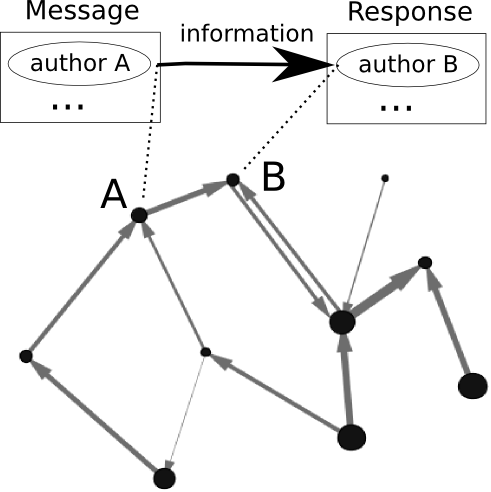
\includegraphics[width=0.3\textwidth]{figs/criaRede__}
	\caption{The formation of interaction networks from email messages. Each vertex represents a participant. A reply message from B to a message from A is regarded as evidence that B has received information from A and yields a directed edge. Multiple messages add ``weight'' to a directed edge. Further details are given in~\cite{evoSN}.}
	\label{fig:formation}
\end{figure}


%\begin{figure}[h!]
%    \centering
%    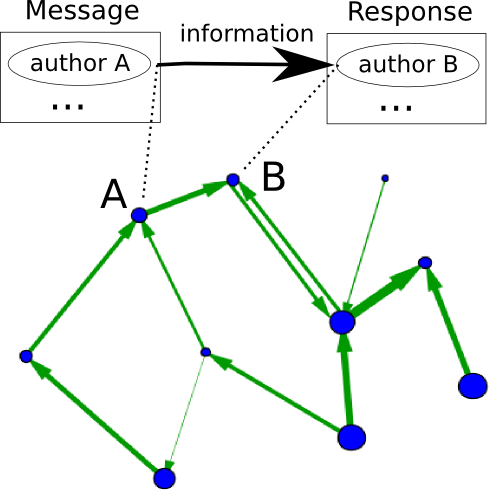
\includegraphics[width=0.3\textwidth]{figs/criaRede_}
%    \caption{Formation of interaction network. Edges are directed as information flows, from
%    an original message's author to the observed responder. Further information is given in Section~\ref{subsec:net}}
%    \label{formationNetwork}
%\end{figure}
%
%Message-response pairs yield interaction networks, such as shown in Figure~\ref{formationNetwork}.
%Each participant is represented by a vertex, and each response is considered evidence that
%information emitted by the first author was received
%by the responder (that had to read, process its contents and render a relevant textual response). Therefore, an edge from first author to the second author (responder) is considered.
%This is the ``information network'' of the system. Edges can be considered in the reverse
%order, from the responder to the original sender, representing status attribution, as the responder
%considered what the sender said worthy of responding and is directing his attention to him. This is the ``status network''. As these networks
%are virtually equivalent, one considers but one of them, usually the information network.

% token size counting
% token type counting
% POS tag via brittle tagger


%\subsection{Network measurements and partitioning}
%The present article uses the same topological measures to observe correlations, PCA formation and network sectioning in peripheral, intermediary and hub sectors,
%Basic network measures of connectivity, in the same networks, were observed in a previous article~\cite{evoSN}.
%The present article uses the same topological measures to observe correlations, PCA formation and network sectioning in peripheral, intermediary and hub sectors,
%through strength measure. As described in that article, the ``exclusivist criteria'' for such partitioning is found to be the closest to literature
%predictions (5\% of hubs, 15\% of intermediary and 80\% of peripheral vertex). Even so, strength-based
%criteria is simpler and yields reasonable results (5-10\%, 5-25\%, 65-90\%).
%Beyond that, changing the sectioning to a degree or a compound criteria did not significantly change the presented results.
%
%Consequently, herein is considered a strength partitioning each sector (periphery, intermediary, hubs) is regarded as a \emph{primitive sector} of the \emph{primitive partitioning}.

%Tests done while mining the data,
%suggested that boudaries should not be considered sharp, but as smooth transitions.

\subsection{Textual measures}
This work focuses on the most simple measures from texts, as they proved sufficient for current step.
%These measures include frequency of individual letters and punctuations (Tables~\ref{tab:cha}), of words and tokens (Table~\ref{tab:tokens}), sizes of tokens, sentences and messages (Table~\ref{tab:sizesTokens},~\ref{tab:sizesSents} and~\ref{tab:sizesMsgs}) and POS (Part-Of-Speech) tags (Table~\ref{tab:pos}). Other measures envisioned are in subsection~\ref{subsec:fw}.
Considered measures are:
\begin{itemize}
    \item Frequency of characters: letters, vowels, punctuations and uppercase.
    \item Number of tokens, frequency of punctuations, of known words, of words that has wordnet synsets, of tokens that are stopwords, of words that return synsets and are stop words, etc.
    \item Mean and standard deviation for word and token sizes.
    \item Mean and standard deviation of sentence sizes.
    \item Mean and standard deviation of message sizes.
    \item Fraction of morphosyntactic classes, such as adverbs, adjectives and nouns, represented by POS (Part-Of-Speech) tags.
\end{itemize}
\noindent To such measures are dedicated Tables~\ref{tab:cha},~\ref{tab:tokens},~\ref{tab:sizesTokens},~\ref{tab:sizesSents},~\ref{tab:sizesMsgs},~\ref{tab:pos}.

This choice is based on: 1) the lack of such information in literature, as far as authors know; 
2) potential relations of these incidences with topological aspects, such as connectivity; 3) the interdependence of textual artifacts suggests that simple measures should reflect complex behaviors and more subtle aspects.
A preliminary study, with the complete works from Machado de Assis, made clear that these measures vary with respect to style~\cite{letrasMachado}.

Wordnet synsets of each word were also used for:
\begin{itemize}
    \item Incidence of hypernyms, hyponyms, holonyms and meronyms.
    \item Use and development of similarity measures of words, phrases and messages, by use of semantic criteria (Wordnet) and bag of words.
\end{itemize}


%\subsection{Topological measures}\label{subsec:top}
%Degree (in, out and total), strength (in, out and total), betweenness centrality and clustering coefficient were measured for each vertex in the interaction network. This served two purposes:
%\begin{itemize}
%    \item Obtaining a sound partitioning of the network in peripheral, intermediary and hub sectors. This was developed in a previous article by the same author~\cite{evoSN}.
%    \item Observance of correlation with textual measures and principal components formation.
%\end{itemize}
%
%These measures are not developed here extensively as they are very consolidated, simple, and was the core of a previous article this subject by the same author~\cite{evoSN}.
%\subsection{Observation of structure}
\subsection{Relating text and topology}\label{sec:ks}
%Key observations for a deeper insight about network structure depend on
%theoretical background and intentions. 
The topological and textual measures were related by:
\begin{enumerate}
    \item incidences of linguistic traces in hub, intermediary and peripheral network sectors, which are delimited by topological criteria.
    \item Correlation of measures of each vertex, easing pattern detection involving topology of interaction and language used.
    \item Principal components formation derived from usual PCA.
\end{enumerate}

%This choice include integration with previous topological results, lack of concise results in literature (as far as author knows) that
%could substantiate correlations of topological and textual traces, and common sense as a long-time member of these networks.
%First task, of textual production in hubs, intermediary and peripheral sectors, is observed by Tables~\ref{tab:cha}-\ref{tab:kolPctInter}.
An adaptation of the Kolmogorov-Smirnov test was used to observe differences in textual content, as follows.
Be $F_{1,n}$ and $F_{2,n'}$ two empirical distribution functions, where $n$ and $n'$ are the number of observations on each sample. The two-sample Kolmogorov-Smirnov test rejects the null hypothesis if:
\begin{equation}\label{eq:ks}
D_{n,n'} > c(\alpha)\sqrt{\frac{n+n'}{nn'}}
\end{equation}

\noindent where $D_{n,n'}=sup_x[F_{1,n}-F_{2,n'}]$ and $c(\alpha)$ is related to the critical region $\alpha$ by:

\begin{table}[H]
\centering
\begin{tabular}{|l||c|c|c|c|c|c|}\hline
$\alpha$    & 0.1  & 0.05 & 0.025 & 0.01 & 0.005 & 0.001 \\\hline
$c(\alpha)$ & 1.22 & 1.36 & 1.48  & 1.63 & 1.73  & 1.95  \\\hline
\end{tabular}
\end{table}

We need to compare empirical distribution functions, therefore $D_{n,n'}$ is given, as are $n$ and $n'$. All terms in equation~\ref{eq:ks} are positive and $c(\alpha)$ can be isolated:

\begin{equation}\label{eq:ks2}
c(\alpha) < \frac{D_{n,n'}}{\sqrt{\frac{n+n'}{nn'}}} = c'(\alpha)
\end{equation}

%Tables~\ref{tab:kolSub}-\ref{tab:kolPctInter} are populated with values for $c'(\alpha)$.
When $c'(\alpha)$ is high, low values of $\alpha$ favor rejecting the null hypothesis.
For example, when $c'(\alpha)$ is greater than $\approx 1.7$, one might assume that $F_{1,n}$ and $F_{2,n'}$ differ.
More importantly for us is that $c'(\alpha)$ is a measure of distance between both distributions~\cite{kolm}.
We use collections of these values for deriving hypotheses
about how different are the underlying mechanisms of the collections.

%Second task is addressed by the correlation matrix with both textual and topological measurements of each participant, in Tables~\ref{tab:corTop}-\ref{tab:corTexTop}. Third, principal components composition are in Tables~\ref{tab:pca1}-\ref{tab:pca5}. 

%For sections (hubs, intermediary and peripheral),
%all messages written by authors in each section were considered together. For the histograms, independent messages were considered from each sector. 
\section{Results and discussion}\label{sec:results}

The most important result in this article is the
extreme differentiation of each Erd\"os sectors with respect to the texts produced.
For example: hubs use more contractions, more adjectives,
more common words, and less punctuation if compared to the rest of the network,
specially the peripheral sector.
In general, the rise or fall of a metric is monotonic along connectivity,
but some of them reached extreme values in the intermediary sector.

Next sections summarize results of immediate interest
and further insights can be obtained by skipping through
the tables and figures in the Supporting Information document.

\subsection{General characteristics of activity distribution among participants}\label{sec:gen}
\begin{table}[h!]
\begin{center}
\begin{tabular}{| l || c | c | c | c |}\hline
 & {\bf g.} & {\bf p.} & {\bf i.} & {\bf h.} \\\hline\hline
$N$ & 17.00  & 7.00  & 6.00  & 4.00 \\
$N_{\%}$ & 100.00  & 41.18  & 35.29  & 23.53 \\\hline
$M$ & 100.00  & 11.00  & 37.00  & 52.00 \\
$M_{\%}$ & 100.00  & 11.00  & 37.00  & 52.00 \\\hline
$\Gamma$ & 18.00  & 4.00  & 8.00  & 6.00 \\
$\Gamma_{\%}$ & 100.00  & 22.22  & 44.44  & 33.33 \\\hline
$\frac{\Gamma}{M}\%$ & 18.00  & 36.36  & 21.62  & 11.54 \\
$\mu(\gamma)$ & 2.67  & 2.50  & 2.75  & 2.67 \\
$\sigma(\gamma)$ & 0.47  & 0.50  & 0.43  & 0.47 \\\hline
\end{tabular}
\caption{Distribution of participants, messages and threads among each Erd\"os sector ({\bf p.} for periphery, {\bf i.} for intermediary, 
    {\bf h.} for hubs) in a total time period of 0.71 years (from 2007-04-24T18:54:28 to 2008-01-10T19:17:26). $N$ is the number of participants, $M$ is the number of messages, $\Gamma$ is the number of threads, and $\gamma$ is the number of messages in a thread.
    The \% denotes the usual `per cent' with respecto to the total quantity ($100\%$ for {\bf g.})
    while $\mu$ and $\sigma$ denote mean and standard deviation.}
\end{center}
\end{table}
Hubs and periphery swap fractions of participants and activity:
while peripheral sector has $\approx 75\%$ of participants, it produces $\approx 10\%$ of all messages.
Conversely, hubs sector present $\approx 10\%$ of participants and produces $\approx 75\%$ of all messages.
% verificar TTM
Fewer threads are created in proportion to total messages sent by the hubs,
while threads created by the periphery are twice as frequent as general peripheral messages.
% medir
This suggests a complementarity between peripheral diversity and hub specialization
which, on its turn, deepens the understanding of the interaction network as a meaningful system, 
notably if yielded by online activity.
These assertions are condensed in Table~\ref{geralListas}.

%Also, comparing lists with a fixed number of messages,
%the number of threads created seem to increase as the number of participants decrease.

\subsection{Characters}\label{sec:cha}
\begin{table}[h!]
\begin{center}
\begin{tabular}{| l || c | c | c | c |}\hline
 & {\bf g.} & {\bf p.} & {\bf i.} & {\bf h.} \\\hline\hline
$chars$ & 82933  & 7162  & 28170  & 47601 \\
$chars_{\%}$ & 100.00  & 8.64  & 33.97  & 57.40 \\\hline
$\frac{spaces}{chars}$ & 14.96  & 13.59  & 15.21  & 15.01 \\
$\frac{punct}{chars-spaces}$ & 8.17  & 6.98  & 8.03  & 8.44 \\
$\frac{digits}{chars-spaces}$ & 0.90  & 1.97  & 0.77  & 0.80 \\\hline
$\frac{letters}{chars-spaces}$ & 88.72  & 88.88  & 88.98  & 88.54 \\
$\frac{vogals}{letters}$ & 40.47  & 39.17  & 40.72  & 40.53 \\
$\frac{uppercase}{letters}$ & 5.27  & 6.22  & 5.39  & 5.05 \\\hline
\end{tabular}
\caption{Characters in each Erd\"os sector ({{\bf p.}} for periphery, {{\bf i.}} for intermediary, 
    {{\bf h.}} for hubs).}
\end{center}
\end{table}
Peripheral vertices use more punctuation characters, digits and uppercase letters.
Hubs use more letters and vowels among letters.
The use of white spaces does not seem to have any relation to connectivity, with the exception that the intermediary presented a slightly lower incidence of spaces than both peripheral and hub sectors. 
The total number of characters in ELE list,
in the 20 thousand messages,
is more than three times what other lists exhibited.
This suggests peculiarities related to communication conventions and style (see Appendix~\ref{sec:materials}) and were found not related to topological features.
Further information is given in Table~\ref{tab:cha}.

\subsection{Tokens and words}\label{subsec:tw}
%\begin{table}[h!]
\begin{center}
\begin{tabular}{| l || c | c | c | c |}\hline
 & {\bf g.} & {\bf p.} & {\bf i.} & {\bf h.} \\\hline\hline
$tokens$ & 17964  & 1539  & 6064  & 10361 \\
$tokens_{\%}$ & 100.00  & 8.57  & 33.76  & 57.68 \\
$tokens \neq$ & 15.21  & 32.16  & 25.89  & 18.02 \\\hline
$\frac{knownw}{tokens}$ & 36.48  & 35.74  & 38.03  & 35.69 \\
$\frac{knownw \neq}{knownw}$ & 8.62  & 24.73  & 15.31  & 10.84 \\\hline
$\frac{stopw}{knownw}$ & 11.43  & 10.00  & 11.71  & 11.47 \\
$\frac{punct}{tokens}$ & 23.73  & 22.35  & 22.82  & 24.47 \\
$\frac{contrac}{tokens}$ & 0.01  & 0.00  & 0.00  & 0.02 \\\hline
\end{tabular}
\caption{tokens in each Erd\"os sector ({{\bf p.}} for periphery, {{\bf i.}} for intermediary, 
    {{\bf h.}} for hubs).}
\end{center}
\end{table}
\begin{table}[h!]
\begin{center}
\begin{tabular}{| l || c | c | c | c |}\hline
 & {\bf g.} & {\bf p.} & {\bf i.} & {\bf h.} \\\hline\hline
$tokens$ & 17964  & 1539  & 6064  & 10361 \\
$tokens_{\%}$ & 100.00  & 8.57  & 33.76  & 57.68 \\
$tokens \neq$ & 15.21  & 32.16  & 25.89  & 18.02 \\\hline
$\frac{knownw}{tokens}$ & 36.48  & 35.74  & 38.03  & 35.69 \\
$\frac{knownw \neq}{knownw}$ & 8.62  & 24.73  & 15.31  & 10.84 \\\hline
$\frac{stopw}{knownw}$ & 11.43  & 10.00  & 11.71  & 11.47 \\
$\frac{punct}{tokens}$ & 23.73  & 22.35  & 22.82  & 24.47 \\
$\frac{contrac}{tokens}$ & 0.01  & 0.00  & 0.00  & 0.02 \\\hline\hline
$\mu(\overline{tokens})$ & 3.84  & 3.94  & 3.86  & 3.82 \\
$\sigma(\overline{tokens})$ & 2.99  & 3.10  & 2.96  & 2.99 \\\hline
$\mu(\overline{knownw})$ & 3.28  & 3.27  & 3.32  & 3.26 \\
$\sigma(\overline{knownw})$ & 1.81  & 1.86  & 1.80  & 1.81 \\\hline
$\mu(\overline{knownw \neq})$ & 5.12  & 4.35  & 4.92  & 4.98 \\
$\sigma(\overline{knownw \neq})$ & 2.20  & 2.22  & 2.25  & 2.15 \\\hline
$\mu(\overline{stopw})$ & 1.77  & 1.84  & 1.77  & 1.76 \\
$\sigma(\overline{stopw})$ & 0.74  & 0.76  & 0.73  & 0.75 \\\hline
\end{tabular}
\caption{Token sizes in each Erd\"os sector ({{\bf p.}} for periphery, {{\bf i.}} for intermediary, {{\bf h.}} for hubs).}
\end{center}
\end{table}

The largest average size of tokens is from the most wordy list (ELE).
This implies that is has more characters, tokens, and characters per token in comparison to the other lists. 
The longer words used by hubs might be related to the use of a specialized vocabulary.
% VERITICCAR TTM
% palavras mais longas podem vir dos perifericos pois nao usam jargao
Although the token diversity ($\frac{|tokens \neq|}{|tokens|}$) found in peripheral sector is far greater, this result has the masking artifact that the peripheral sector corpus is smaller, yielding a larger token diversity.
% medir para tamanhos equivalentes de texto TTM
This can be noticed by the token diversity of the whole network, which is lower than in any of the sections.
This same results apply to the lexical diversity ($\frac{|kw\neq|}{kw}$).

Punctuations among tokens are less abundant in hubs, and discrepancies here are larger than with characters comparisons (subsection~\ref{sec:cha}). Known words are used more frequently by hubs.

ELE and CPP both exhibit intermediaries 
with the more frequent production of punctuation,
less frequent production of known words, and
the highest incidence of words with wordnet synsets among known words.
This suggests some peculiarity in network structure,
such as authorities in the intermediary sector of such networks,
using smaller sentences and a more intensive use of jargons,
as made explicit in the following sections.
% verificar isso e ver o que fazer

Words with synsets,
among known English words, are less frequent in hubs sector,
further evidencing the jargon and specialization hubs develop.
% verificar, desenvolvar

Further information is given in Table~\ref{tab:tokens}.

\subsection{Sizes of tokens and words}\label{subsec:tw2}
%\begin{table}[h!]
\begin{center}
\begin{tabular}{| l || c | c | c | c |}\hline
 & {\bf g.} & {\bf p.} & {\bf i.} & {\bf h.} \\\hline\hline
$\mu(\overline{tokens})$ & 3.84  & 3.94  & 3.86  & 3.82 \\
$\sigma(\overline{tokens})$ & 2.99  & 3.10  & 2.96  & 2.99 \\\hline
$\mu(\overline{knownw})$ & 3.28  & 3.27  & 3.32  & 3.26 \\
$\sigma(\overline{knownw})$ & 1.81  & 1.86  & 1.80  & 1.81 \\\hline
$\mu(\overline{knownw \neq})$ & 5.12  & 4.35  & 4.92  & 4.98 \\
$\sigma(\overline{knownw \neq})$ & 2.20  & 2.22  & 2.25  & 2.15 \\\hline
$\mu(\overline{stopw})$ & 1.77  & 1.84  & 1.77  & 1.76 \\
$\sigma(\overline{stopw})$ & 0.74  & 0.76  & 0.73  & 0.75 \\\hline
\end{tabular}
\caption{Token sizes in each Erd\"os sector ({{\bf p.}} for periphery, {{\bf i.}} for intermediary, {{\bf h.}} for hubs).}
\end{center}
\end{table}
Sizes of known words are smaller for hubs, which suggests its use of more common words, although some of the previous results suggests that hubs have a very differentiated and specialized vocabulary. 
Larger words seems to be related to intermediary sector,
which might be related to the use of elaborated vocabulary.
Further details are given in Table~\ref{tab:sizesTokens}.

\subsection{Sizes of sentences}\label{subsec:ss}
\begin{table}[h!]
\begin{center}
\begin{tabular}{| l || c | c | c | c |}\hline
 & {\bf g.} & {\bf p.} & {\bf i.} & {\bf h.} \\\hline\hline
$sents$ & 558  & 45  & 211  & 304 \\
$sents_{\%}$ & 99.64  & 8.04  & 37.68  & 54.29 \\\hline
$\mu_S(chars)$ & 147.51  & 158.07  & 132.44  & 155.44 \\
$\sigma_S(chars)$ & 147.95  & 154.11  & 135.56  & 154.01 \\\hline
$\mu_S(tokens)$ & 32.21  & 34.22  & 28.75  & 34.09 \\
$\sigma_S(tokens)$ & 32.08  & 32.64  & 29.17  & 33.60 \\\hline
$\mu_S(knownw)$ & 9.90  & 9.82  & 9.10  & 10.39 \\
$\sigma_S(knownw)$ & 10.37  & 11.34  & 9.14  & 10.92 \\\hline
$\mu_S(stopw)$ & 1.18  & 1.11  & 1.15  & 1.20 \\
$\sigma_S(stopw)$ & 1.57  & 1.22  & 1.52  & 1.64 \\\hline
$\mu_S(puncts)$ & 7.65  & 7.67  & 6.57  & 8.35 \\
$\sigma_S(puncts)$ & 11.30  & 8.19  & 10.69  & 11.98 \\\hline
\end{tabular}
\caption{Sentences sizes in each Erd\"os sector ({{\bf p.}} for periphery, {{\bf i.}} for intermediary, {{\bf h.}} for hubs).}
\end{center}
\end{table}
Hubs present the lowest average sentence size,
both in characters and in tokens.
We hypothesize that this smaller sentence use
is related to the efficiency of hub specialization.
Also, the incidence of usual known words seems to decay with connectivity, as does the number of known words with wordnet synsets.
This reflects our view that connectivity is inversely proportional
to diversity.

Further information is given in Table~\ref{tab:sizesSents}.

\subsection{Messages}\label{subsec:mm}
\begin{table}[h!]
\begin{center}
\begin{tabular}{| l || c | c | c | c |}\hline
 & {\bf g.} & {\bf p.} & {\bf i.} & {\bf h.} \\\hline\hline
$msgs$ & 100  & 11  & 37  & 52 \\
$msgs_{\%}$ & 100.00  & 11.00  & 37.00  & 52.00 \\\hline
$\mu_M(sents)$ & 6.54  & 4.91  & 6.62  & 6.83 \\
$\sigma_M(sents)$ & 5.09  & 3.26  & 6.28  & 4.35 \\\hline
$\mu_M(tokens)$ & 179.79  & 140.00  & 163.97  & 199.46 \\
$\sigma_M(tokens)$ & 183.42  & 71.56  & 182.94  & 197.24 \\\hline
$\mu_M(knownw)$ & 55.24  & 40.18  & 51.92  & 60.79 \\
$\sigma_M(knownw)$ & 61.67  & 26.49  & 59.82  & 67.33 \\\hline
$\mu_M(stopw)$ & 6.55  & 4.55  & 6.54  & 6.98 \\
$\sigma_M(stopw)$ & 6.92  & 3.11  & 7.11  & 7.29 \\\hline
$\mu_M(puncts)$ & 42.77  & 31.36  & 37.46  & 48.96 \\
$\sigma_M(puncts)$ & 48.91  & 14.92  & 48.61  & 52.78 \\\hline
$\mu_M(chars)$ & 829.31  & 651.09  & 761.35  & 915.37 \\
$\sigma_M(chars)$ & 878.54  & 342.18  & 889.47  & 937.65 \\\hline
\end{tabular}
\caption{Messages sizes in each Erd\"os sector ({{\bf p.}} for periphery, {{\bf i.}} for intermediary, {{\bf h.}} for hubs).}
\end{center}
\end{table}
Connectivity was related to smaller messages in terms of characters and tokens.
% tirar medidas de correlacao: perason e spearmanA TTM
ELE list displayed an inverse situation:
the more connected the sector,
the longer the messages are.
This was considered a peculiarity of the culture bonded
with the political subject of ELE list, to be further verified.
% make some sort of verification TTM
% process the lists just for this feature
Regarding sentences,
the size of messages seem to hold steady throughout connectivity.
% ver a correlação das medidas de grau e força com TTM
% texto
% ver em especial se algo eh mais para in ou out
% e se indifere greu e força como no particionamento de erdos
Further information is given in Table~\ref{tab:sizesMsgs}.

\subsection{POS tags}\label{subsec:pos}
\begin{table}[h!]
\begin{center}
\begin{tabular}{| l || c | c | c | c |}\hline
 & {\bf g.} & {\bf p.} & {\bf i.} & {\bf h.} \\\hline\hline
NOUN & 56.40  & 58.68  & 55.67  & 56.50 \\
X & 16.46  & 16.20  & 16.58  & 16.42 \\\hline
ADP & 7.22  & 6.78  & 7.38  & 7.18 \\
DET & 6.07  & 5.12  & 6.41  & 6.02 \\\hline
VERB & 5.13  & 4.46  & 5.90  & 4.75 \\\hline
ADJ & 3.29  & 3.97  & 2.87  & 3.44 \\
ADV & 2.07  & 2.15  & 1.82  & 2.21 \\\hline
PRT & 1.79  & 1.32  & 1.51  & 2.04 \\
PRON & 1.18  & 0.83  & 1.48  & 1.04 \\
NUM & 0.33  & 0.50  & 0.27  & 0.34 \\
CONJ & 0.07  & 0.00  & 0.12  & 0.05 \\
PUNC & 0.00  & 0.00  & 0.00  & 0.00 \\\hline
\end{tabular}
\caption{POS tags in each Erd\"os sector ({{\bf p.}} for periphery, {{\bf i.}} for intermediary, {{\bf h.}} for hubs).
    Universal POS tags~\cite{{petrov}}:
    VERB - verbs (all tenses and modes);
    NOUN - nouns (common and proper);
    PRON - pronouns;
    ADJ - adjectives;
    ADV - adverbs;
    ADP - adpositions (prepositions and postpositions);
    CONJ - conjunctions;
    DET - determiners;
    NUM - cardinal numbers;
    PRT - particles or other function words;
    X - other: foreign words, typos, abbreviations;
    PUNCT - punctuation.
}
\end{center}
\end{table}
% rever taggeamento e tentar melhor accuracy com o Bril Tagger TTM
Lower connectivity yields more nouns and less adjectives,
adverbs and verbs.
This suggests that the networks collect issues important
to the world by the peripheral sector. 
These issues are qualified, elaborated about,
by the more connected participants.
This is a further indicative that peripheral sectors
are related to diversity while hubs relate to specialization.
Further information is given in Table~\ref{tab:pos}.

\subsection{Wordnet synsets}\label{subsec:pos}
\begin{table}[h!]
\begin{center}
\begin{tabular}{| l || c | c | c | c |}\hline
 & {\bf g.} & {\bf p.} & {\bf i.} & {\bf h.} \\\hline\hline
N & 88.79  & 91.15  & 87.41  & 89.26 \\\hline
ADJ & 6.11  & 7.08  & 5.34  & 6.42 \\\hline
VERB & 0.24  & 0.00  & 0.38  & 0.19 \\\hline
ADV & 4.86  & 1.77  & 6.86  & 4.13 \\\hline\hline
POS & 21.05  & 22.01  & 21.61  & 20.58 \\\hline
POS! & 72.54  & 74.83  & 71.48  & 72.85 \\\hline
\end{tabular}
\caption{Percentage of synsets with each of the POS tags used by Wordnet. The last lines give the percentage of words considered from all of the tokens (POS) and from the words with synset (POS!). The tokens not considered are punctuations, unrecognized words, words without synsets, stopwords and words for which Wordnet has no synset  tagged with POS tags . Values for each Erd\"os sectors are in the columns {{\bf p.}} for periphery, {{\bf i.}} for intermediary, {{\bf h.}} for hubs.}
\end{center}
\end{table} % uma soh
%\begin{table}[h!]
\begin{center}
\begin{tabular}{| l || c | c | c | c |}\hline
 & {\bf g.} & {\bf p.} & {\bf i.} & {\bf h.} \\\hline\hline
$\mu(min\,depth)$ & 5.87  & 5.90  & 5.82  & 5.90 \\
$\sigma(min\,depth)$ & 2.62  & 2.40  & 2.68  & 2.61 \\\hline
$\mu(max\,depth)$ & 6.31  & 6.42  & 6.24  & 6.34 \\
$\sigma(max\,depth)$ & 2.85  & 2.66  & 2.91  & 2.83 \\\hline
$\mu(holonyms)$ & 0.57  & 0.67  & 0.57  & 0.56 \\
$\sigma(holonyms)$ & 1.34  & 1.43  & 1.32  & 1.34 \\\hline
$\mu(meronyms)$ & 0.96  & 0.76  & 0.75  & 1.12 \\
$\sigma(meronyms)$ & 4.40  & 2.61  & 3.77  & 4.95 \\\hline
$\mu(domains)$ & 0.08  & 0.06  & 0.10  & 0.06 \\
$\sigma(domains)$ & 0.27  & 0.25  & 0.31  & 0.25 \\\hline
$\mu(similar)$ & 0.26  & 0.28  & 0.19  & 0.30 \\
$\sigma(similar)$ & 1.50  & 1.39  & 1.11  & 1.71 \\\hline
$\mu(verb\,groups)$ & 0.01  & 0.01  & 0.02  & 0.01 \\
$\sigma(verb\,groups)$ & 0.12  & 0.09  & 0.14  & 0.11 \\\hline
$\mu(lemmas)$ & 3.03  & 2.73  & 3.17  & 2.99 \\
$\sigma(lemmas)$ & 2.13  & 1.73  & 2.29  & 2.09 \\\hline
$\mu(entailments)$ & 0.01  & 0.00  & 0.01  & 0.00 \\
$\sigma(entailments)$ & 0.08  & 0.00  & 0.10  & 0.06 \\\hline
$\mu(hyponyms)$ & 3.35  & 3.06  & 3.19  & 3.50 \\
$\sigma(hyponyms)$ & 12.82  & 20.25  & 8.56  & 13.46 \\\hline
$\mu(hypernyms)$ & 1.00  & 1.01  & 1.00  & 1.00 \\
$\sigma(hypernyms)$ & 0.40  & 0.43  & 0.38  & 0.41 \\\hline
\end{tabular}
\caption{Measures of wordnet features in each Erd\"os sector ({{\bf p.}} for periphery, {{\bf i.}} for intermediary, {{\bf h.}} for hubs).}
\end{center}
\end{table} % uma soh


% POS -> n
% fname -> /home/r/repos/artigoTextoNasRedes/tables/wnPOSInline2-n_.tex
\begin{table}[h!]
\begin{center}
\begin{tabular}{| l || c | c | c | c |}\hline
 & {\bf g.} & {\bf p.} & {\bf i.} & {\bf h.} \\\hline\hline
$\mu(min\,depth)$ & 6.52  & 6.41  & 6.52  & 6.53 \\
$\sigma(min\,depth)$ & 1.94  & 1.77  & 2.01  & 1.93 \\\hline
$\mu(max\,depth)$ & 7.02  & 6.99  & 7.00  & 7.03 \\
$\sigma(max\,depth)$ & 2.13  & 1.99  & 2.20  & 2.11 \\\hline
$\mu(holonyms)$ & 0.65  & 0.73  & 0.65  & 0.63 \\
$\sigma(holonyms)$ & 1.41  & 1.48  & 1.39  & 1.40 \\\hline
$\mu(meronyms)$ & 1.08  & 0.83  & 0.86  & 1.25 \\
$\sigma(meronyms)$ & 4.66  & 2.72  & 4.02  & 5.22 \\\hline
$\mu(domains)$ & 0.07  & 0.07  & 0.10  & 0.06 \\
$\sigma(domains)$ & 0.27  & 0.26  & 0.30  & 0.25 \\\hline
$\mu(similar)$ & 0.00  & 0.00  & 0.00  & 0.00 \\
$\sigma(similar)$ & 0.00  & 0.00  & 0.00  & 0.00 \\\hline
$\mu(verb\,groups)$ & 0.00  & 0.00  & 0.00  & 0.00 \\
$\sigma(verb\,groups)$ & 0.00  & 0.00  & 0.00  & 0.00 \\\hline
$\mu(lemmas)$ & 3.07  & 2.80  & 3.19  & 3.04 \\
$\sigma(lemmas)$ & 2.14  & 1.74  & 2.32  & 2.08 \\\hline
$\mu(entailments)$ & 0.00  & 0.00  & 0.00  & 0.00 \\
$\sigma(entailments)$ & 0.00  & 0.00  & 0.00  & 0.00 \\\hline
$\mu(hyponyms)$ & 3.42  & 3.30  & 3.02  & 3.68 \\
$\sigma(hyponyms)$ & 13.17  & 21.19  & 7.42  & 14.14 \\\hline
$\mu(hypernyms)$ & 1.09  & 1.09  & 1.08  & 1.09 \\
$\sigma(hypernyms)$ & 0.30  & 0.34  & 0.28  & 0.31 \\\hline
\end{tabular}
\caption{Measures of wordnet features in each Erd\"os sector ({{\bf p.}} for periphery, {{\bf i.}} for intermediary, {{\bf h.}} for hubs).}
\end{center}
\end{table}
% fname -> /home/r/repos/artigoTextoNasRedes/tables/wnPOSInline2a-n_.tex
\begin{table}[h!]
\begin{center}
\begin{tabular}{| l || c | c | c | c |}\hline
 & {\bf g.} & {\bf p.} & {\bf i.} & {\bf h.} \\\hline\hline
entity.n.01 & 100.00  & 100.00  & 100.00  & 100.00 \\\hline\hline
{{\bf total}} & 100.00  & 100.00  & 100.00  & 100.00 \\\hline
\end{tabular}
\caption{Counts for the most incident synsets at the semantic roots in each Erd\"os sector ({\bf p.} for periphery, {\bf i.} for intermediary, {\bf h.} for hubs). Yes.}
\end{center}
\end{table}
% fname -> /home/r/repos/artigoTextoNasRedes/tables/wnPOSInline2b-n_.tex
\begin{table}[h!]
\begin{center}
\begin{tabular}{| l || c | c | c | c |}\hline
 & {\bf g.} & {\bf p.} & {\bf i.} & {\bf h.} \\\hline\hline
abstraction.n.06 & 58.86  & 62.14  & 55.58  & 60.29 \\\hline
physical\_entity.n.01 & 41.14  & 37.86  & 44.42  & 39.71 \\\hline\hline
{{\bf total}} & 100.00  & 100.00  & 100.00  & 100.00 \\\hline
\end{tabular}
\caption{Counts for the most incident synsets one step from the semantic roots in each Erd\"os sector ({\bf p.} for periphery, {\bf i.} for intermediary, {\bf h.} for hubs).}
\end{center}
\end{table}
% fname -> /home/r/repos/artigoTextoNasRedes/tables/wnPOSInline2c-n_.tex
\begin{table}[h!]
\begin{center}
\begin{tabular}{| l || c | c | c | c |}\hline
 & {\bf g.} & {\bf p.} & {\bf i.} & {\bf h.} \\\hline\hline
matter.n.03 & 24.03  & 22.33  & 24.96  & 23.74 \\\hline
communication.n.02 & 11.97  & 15.86  & 11.26  & 11.76 \\\hline
group.n.01 & 11.70  & 13.59  & 9.42  & 12.76 \\\hline
relation.n.01 & 10.12  & 9.39  & 9.51  & 10.61 \\\hline
object.n.01 & 8.99  & 4.85  & 11.08  & 8.40 \\\hline
psychological\_feature.n.01 & 8.99  & 6.80  & 8.55  & 9.61 \\\hline
measure.n.02 & 8.43  & 7.77  & 9.42  & 7.93 \\\hline
attribute.n.02 & 7.65  & 8.74  & 7.42  & 7.62 \\\hline
causal\_agent.n.01 & 5.06  & 7.12  & 5.15  & 4.67 \\\hline
thing.n.12 & 3.04  & 3.24  & 3.23  & 2.89 \\\hline
process.n.06 & 0.03  & 0.32  & 0.00  & 0.00 \\\hline\hline
{{\bf total}} & 100.00  & 100.00  & 100.00  & 100.00 \\\hline
\end{tabular}
\caption{Counts for the most incident synsets two step from the semantic roots in each Erd\"os sector ({\bf p.} for periphery, {\bf i.} for intermediary, {\bf h.} for hubs).}
\end{center}
\end{table}
% fname -> /home/r/repos/artigoTextoNasRedes/tables/wnPOSInline2d-n_.tex
\begin{table}[h!]
\begin{center}
\begin{tabular}{| l || c | c | c | c |}\hline
 & {\bf g.} & {\bf p.} & {\bf i.} & {\bf h.} \\\hline\hline
substance.n.01 & 26.49  & 26.15  & 27.39  & 26.01 \\\hline
position.n.07 & 10.58  & 9.62  & 10.37  & 10.86 \\\hline
definite\_quantity.n.01 & 8.40  & 5.77  & 9.23  & 8.32 \\\hline
state.n.02 & 8.25  & 10.00  & 8.30  & 7.95 \\\hline
event.n.01 & 7.62  & 5.77  & 7.16  & 8.19 \\\hline
whole.n.02 & 7.37  & 2.69  & 9.23  & 7.01 \\\hline
social\_group.n.01 & 7.05  & 9.23  & 5.71  & 7.51 \\\hline
written\_communication.n.01 & 6.98  & 8.85  & 5.91  & 7.32 \\\hline
person.n.01 & 5.71  & 8.08  & 5.91  & 5.21 \\\hline
message.n.02 & 5.29  & 8.46  & 4.36  & 5.34 \\\hline
body\_of\_water.n.01 & 3.21  & 3.08  & 3.42  & 3.10 \\\hline
cognition.n.01 & 3.03  & 2.31  & 3.01  & 3.17 \\\hline\hline
{{\bf total}} & 100.00  & 100.00  & 100.00  & 100.00 \\\hline
\end{tabular}
\caption{Counts for the most incident synsets three step from the semantic roots in each Erd\"os sector ({\bf p.} for periphery, {\bf i.} for intermediary, {\bf h.} for hubs).}
\end{center}
\end{table}

% POS -> as
% fname -> /home/r/repos/artigoTextoNasRedes/tables/wnPOSInline2-as_.tex
\begin{table}[h!]
\begin{center}
\begin{tabular}{| l || c | c | c | c |}\hline
 & {\bf g.} & {\bf p.} & {\bf i.} & {\bf h.} \\\hline\hline
$\mu(min\,depth)$ & 0.00  & 0.00  & 0.00  & 0.00 \\
$\sigma(min\,depth)$ & 0.00  & 0.00  & 0.00  & 0.00 \\\hline
$\mu(max\,depth)$ & 0.00  & 0.00  & 0.00  & 0.00 \\
$\sigma(max\,depth)$ & 0.00  & 0.00  & 0.00  & 0.00 \\\hline
$\mu(holonyms)$ & 0.00  & 0.00  & 0.00  & 0.00 \\
$\sigma(holonyms)$ & 0.00  & 0.00  & 0.00  & 0.00 \\\hline
$\mu(meronyms)$ & 0.00  & 0.00  & 0.00  & 0.00 \\
$\sigma(meronyms)$ & 0.00  & 0.00  & 0.00  & 0.00 \\\hline
$\mu(domains)$ & 0.02  & 0.00  & 0.03  & 0.02 \\
$\sigma(domains)$ & 0.15  & 0.00  & 0.17  & 0.15 \\\hline
$\mu(similar)$ & 4.29  & 4.00  & 3.63  & 4.68 \\
$\sigma(similar)$ & 4.41  & 3.50  & 3.25  & 4.99 \\\hline
$\mu(verb\,groups)$ & 0.00  & 0.00  & 0.00  & 0.00 \\
$\sigma(verb\,groups)$ & 0.00  & 0.00  & 0.00  & 0.00 \\\hline
$\mu(lemmas)$ & 2.07  & 2.08  & 2.49  & 1.85 \\
$\sigma(lemmas)$ & 1.79  & 1.50  & 2.06  & 1.64 \\\hline
$\mu(entailments)$ & 0.00  & 0.00  & 0.00  & 0.00 \\
$\sigma(entailments)$ & 0.00  & 0.00  & 0.00  & 0.00 \\\hline
$\mu(hyponyms)$ & 0.00  & 0.00  & 0.00  & 0.00 \\
$\sigma(hyponyms)$ & 0.00  & 0.00  & 0.00  & 0.00 \\\hline
$\mu(hypernyms)$ & 0.00  & 0.00  & 0.00  & 0.00 \\
$\sigma(hypernyms)$ & 0.00  & 0.00  & 0.00  & 0.00 \\\hline
\end{tabular}
\caption{Measures of wordnet features in each Erd\"os sector ({{\bf p.}} for periphery, {{\bf i.}} for intermediary, {{\bf h.}} for hubs).}
\end{center}
\end{table}
% fname -> /home/r/repos/artigoTextoNasRedes/tables/wnPOSInline2a-as_.tex
\begin{table}[h!]
\begin{center}
\begin{tabular}{| l || c | c | c | c |}\hline
 & {\bf g.} & {\bf p.} & {\bf i.} & {\bf h.} \\\hline\hline
public.a.01 & 40.34  & 57.14  & 33.33  & 40.59 \\\hline
temporal.s.01 & 16.48  & 0.00  & 11.11  & 22.77 \\\hline
chief.s.01 & 13.64  & 0.00  & 24.07  & 10.89 \\\hline
new.a.01 & 6.25  & 4.76  & 1.85  & 8.91 \\\hline
global.s.01 & 4.55  & 9.52  & 5.56  & 2.97 \\\hline
ocular.a.02 & 3.98  & 19.05  & 1.85  & 1.98 \\\hline
variable.a.01 & 3.41  & 0.00  & 1.85  & 4.95 \\\hline
impermanent.a.01 & 2.84  & 0.00  & 5.56  & 1.98 \\\hline
simple.a.01 & 2.27  & 4.76  & 3.70  & 0.99 \\\hline
alive.a.01 & 2.27  & 0.00  & 7.41  & 0.00 \\\hline
standard.a.01 & 2.27  & 0.00  & 0.00  & 3.96 \\\hline
virtual.s.01 & 1.70  & 4.76  & 3.70  & 0.00 \\\hline\hline
{{\bf total}} & 100.00  & 100.00  & 100.00  & 100.00 \\\hline
\end{tabular}
\caption{Counts for the most incident synsets at the semantic roots in each Erd\"os sector ({\bf p.} for periphery, {\bf i.} for intermediary, {\bf h.} for hubs). Yes.}
\end{center}
\end{table}

% POS -> v
% fname -> /home/r/repos/artigoTextoNasRedes/tables/wnPOSInline2-v_.tex
\begin{table}[h!]
\begin{center}
\begin{tabular}{| l || c | c | c | c |}\hline
 & {\bf g.} & {\bf p.} & {\bf i.} & {\bf h.} \\\hline\hline
$\mu(min\,depth)$ & 1.72  & 2.83  & 1.70  & 1.66 \\
$\sigma(min\,depth)$ & 1.38  & 1.77  & 1.17  & 1.51 \\\hline
$\mu(max\,depth)$ & 1.72  & 2.83  & 1.70  & 1.66 \\
$\sigma(max\,depth)$ & 1.38  & 1.77  & 1.17  & 1.51 \\\hline
$\mu(holonyms)$ & 0.00  & 0.00  & 0.00  & 0.00 \\
$\sigma(holonyms)$ & 0.00  & 0.00  & 0.00  & 0.00 \\\hline
$\mu(meronyms)$ & 0.00  & 0.00  & 0.00  & 0.00 \\
$\sigma(meronyms)$ & 0.00  & 0.00  & 0.00  & 0.00 \\\hline
$\mu(domains)$ & 0.21  & 0.00  & 0.26  & 0.18 \\
$\sigma(domains)$ & 0.41  & 0.00  & 0.44  & 0.39 \\\hline
$\mu(similar)$ & 0.00  & 0.00  & 0.00  & 0.00 \\
$\sigma(similar)$ & 0.00  & 0.00  & 0.00  & 0.00 \\\hline
$\mu(verb\,groups)$ & 0.23  & 0.50  & 0.22  & 0.23 \\
$\sigma(verb\,groups)$ & 0.48  & 0.50  & 0.49  & 0.47 \\\hline
$\mu(lemmas)$ & 3.42  & 1.67  & 3.49  & 3.48 \\
$\sigma(lemmas)$ & 2.09  & 0.75  & 1.97  & 2.23 \\\hline
$\mu(entailments)$ & 0.12  & 0.00  & 0.16  & 0.09 \\
$\sigma(entailments)$ & 0.32  & 0.00  & 0.36  & 0.29 \\\hline
$\mu(hyponyms)$ & 6.52  & 3.00  & 7.97  & 5.27 \\
$\sigma(hyponyms)$ & 13.64  & 2.71  & 18.33  & 6.38 \\\hline
$\mu(hypernyms)$ & 0.78  & 0.83  & 0.82  & 0.73 \\
$\sigma(hypernyms)$ & 0.42  & 0.37  & 0.38  & 0.45 \\\hline
\end{tabular}
\caption{Measures of wordnet features in each Erd\"os sector ({{\bf p.}} for periphery, {{\bf i.}} for intermediary, {{\bf h.}} for hubs).}
\end{center}
\end{table}
% fname -> /home/r/repos/artigoTextoNasRedes/tables/wnPOSInline2a-v_.tex
\begin{table}[h!]
\begin{center}
\begin{tabular}{| l || c | c | c | c |}\hline
 & {\bf g.} & {\bf p.} & {\bf i.} & {\bf h.} \\\hline\hline
think.v.03 & 24.52  & 0.00  & 25.00  & 25.33 \\\hline
act.v.01 & 16.13  & 75.00  & 13.16  & 16.00 \\\hline
change.v.01 & 12.26  & 0.00  & 11.84  & 13.33 \\\hline
change.v.02 & 11.61  & 25.00  & 11.84  & 10.67 \\\hline
include.v.01 & 9.68  & 0.00  & 10.53  & 9.33 \\\hline
make.v.03 & 7.74  & 0.00  & 11.84  & 4.00 \\\hline
affect.v.05 & 3.23  & 0.00  & 2.63  & 4.00 \\\hline
work.v.01 & 3.23  & 0.00  & 0.00  & 6.67 \\\hline
be.v.01 & 3.23  & 0.00  & 1.32  & 5.33 \\\hline
travel.v.01 & 3.23  & 0.00  & 5.26  & 1.33 \\\hline
use.v.01 & 2.58  & 0.00  & 3.95  & 1.33 \\\hline
insist.v.01 & 2.58  & 0.00  & 2.63  & 2.67 \\\hline\hline
{{\bf total}} & 100.00  & 100.00  & 100.00  & 100.00 \\\hline
\end{tabular}
\caption{Counts for the most incident synsets at the semantic roots in each Erd\"os sector ({\bf p.} for periphery, {\bf i.} for intermediary, {\bf h.} for hubs). Yes.}
\end{center}
\end{table}
% fname -> /home/r/repos/artigoTextoNasRedes/tables/wnPOSInline2b-v_.tex
\begin{table}[h!]
\begin{center}
\begin{tabular}{| l || c | c | c | c |}\hline
 & {\bf g.} & {\bf p.} & {\bf i.} & {\bf h.} \\\hline\hline
reason.v.01 & 27.73  & 0.00  & 28.33  & 28.57 \\\hline
change\_shape.v.01 & 13.45  & 0.00  & 13.33  & 14.29 \\\hline
end.v.02 & 13.45  & 0.00  & 13.33  & 14.29 \\\hline
interact.v.01 & 13.45  & 100.00  & 10.00  & 12.50 \\\hline
try.v.01 & 7.56  & 0.00  & 6.67  & 8.93 \\\hline
create\_verbally.v.01 & 5.04  & 0.00  & 10.00  & 0.00 \\\hline
surprise.v.01 & 4.20  & 0.00  & 3.33  & 5.36 \\\hline
assert.v.01 & 3.36  & 0.00  & 3.33  & 3.57 \\\hline
evaluate.v.02 & 3.36  & 0.00  & 3.33  & 3.57 \\\hline
specify.v.03 & 3.36  & 0.00  & 1.67  & 5.36 \\\hline
return.v.01 & 2.52  & 0.00  & 3.33  & 1.79 \\\hline
discard.v.01 & 2.52  & 0.00  & 3.33  & 1.79 \\\hline\hline
{{\bf total}} & 100.00  & 100.00  & 100.00  & 100.00 \\\hline
\end{tabular}
\caption{Counts for the most incident synsets one step from the semantic roots in each Erd\"os sector ({\bf p.} for periphery, {\bf i.} for intermediary, {\bf h.} for hubs).}
\end{center}
\end{table}
% fname -> /home/r/repos/artigoTextoNasRedes/tables/wnPOSInline2c-v_.tex
\begin{table}[h!]
\begin{center}
\begin{tabular}{| l || c | c | c | c |}\hline
 & {\bf g.} & {\bf p.} & {\bf i.} & {\bf h.} \\\hline\hline
deduce.v.01 & 32.67  & 0.00  & 32.69  & 35.56 \\\hline
start.v.14 & 15.84  & 0.00  & 15.38  & 17.78 \\\hline
interrupt.v.04 & 15.84  & 0.00  & 15.38  & 17.78 \\\hline
relate.v.05 & 9.90  & 25.00  & 9.62  & 8.89 \\\hline
write.v.01 & 5.94  & 0.00  & 11.54  & 0.00 \\\hline
catch.v.01 & 4.95  & 0.00  & 3.85  & 6.67 \\\hline
communicate.v.02 & 3.96  & 50.00  & 0.00  & 4.44 \\\hline
dump.v.01 & 2.97  & 0.00  & 3.85  & 2.22 \\\hline
treat.v.01 & 1.98  & 0.00  & 1.92  & 2.22 \\\hline
name.v.01 & 1.98  & 0.00  & 3.85  & 0.00 \\\hline
correct.v.01 & 1.98  & 25.00  & 1.92  & 0.00 \\\hline
represent.v.09 & 1.98  & 0.00  & 0.00  & 4.44 \\\hline\hline
{{\bf total}} & 100.00  & 100.00  & 100.00  & 100.00 \\\hline
\end{tabular}
\caption{Counts for the most incident synsets two step from the semantic roots in each Erd\"os sector ({\bf p.} for periphery, {\bf i.} for intermediary, {\bf h.} for hubs).}
\end{center}
\end{table}
% fname -> /home/r/repos/artigoTextoNasRedes/tables/wnPOSInline2d-v_.tex
\begin{table}[h!]
\begin{center}
\begin{tabular}{| l || c | c | c | c |}\hline
 & {\bf g.} & {\bf p.} & {\bf i.} & {\bf h.} \\\hline\hline
disrespect.v.01 & 35.71  & 25.00  & 45.45  & 30.77 \\\hline
inform.v.01 & 14.29  & 50.00  & 0.00  & 15.38 \\\hline
map.v.01 & 7.14  & 0.00  & 0.00  & 15.38 \\\hline
object.v.01 & 7.14  & 0.00  & 9.09  & 7.69 \\\hline
ignore.v.01 & 7.14  & 0.00  & 9.09  & 7.69 \\\hline
prefer.v.03 & 7.14  & 0.00  & 18.18  & 0.00 \\\hline
debug.v.01 & 7.14  & 25.00  & 9.09  & 0.00 \\\hline
double.v.01 & 3.57  & 0.00  & 0.00  & 7.69 \\\hline
adhere.v.06 & 3.57  & 0.00  & 0.00  & 7.69 \\\hline
program.v.01 & 3.57  & 0.00  & 0.00  & 7.69 \\\hline
roll\_up.v.02 & 3.57  & 0.00  & 9.09  & 0.00 \\\hline\hline
{{\bf total}} & 100.00  & 100.00  & 100.00  & 100.00 \\\hline
\end{tabular}
\caption{Counts for the most incident synsets three step from the semantic roots in each Erd\"os sector ({\bf p.} for periphery, {\bf i.} for intermediary, {\bf h.} for hubs).}
\end{center}
\end{table}

% POS -> r
% fname -> /home/r/repos/artigoTextoNasRedes/tables/wnPOSInline2-r_.tex
\begin{table}[h!]
\begin{center}
\begin{tabular}{| l || c | c | c | c |}\hline
 & {\bf g.} & {\bf p.} & {\bf i.} & {\bf h.} \\\hline\hline
$\mu(min\,depth)$ & 0.00  & nan  & 0.00  & 0.00 \\
$\sigma(min\,depth)$ & 0.00  & nan  & 0.00  & 0.00 \\\hline
$\mu(max\,depth)$ & 0.00  & nan  & 0.00  & 0.00 \\
$\sigma(max\,depth)$ & 0.00  & nan  & 0.00  & 0.00 \\\hline
$\mu(holonyms)$ & 0.00  & nan  & 0.00  & 0.00 \\
$\sigma(holonyms)$ & 0.00  & nan  & 0.00  & 0.00 \\\hline
$\mu(meronyms)$ & 0.00  & nan  & 0.00  & 0.00 \\
$\sigma(meronyms)$ & 0.00  & nan  & 0.00  & 0.00 \\\hline
$\mu(domains)$ & 0.11  & nan  & 0.20  & 0.00 \\
$\sigma(domains)$ & 0.31  & nan  & 0.40  & 0.00 \\\hline
$\mu(similar)$ & 0.00  & nan  & 0.00  & 0.00 \\
$\sigma(similar)$ & 0.00  & nan  & 0.00  & 0.00 \\\hline
$\mu(verb\,groups)$ & 0.00  & nan  & 0.00  & 0.00 \\
$\sigma(verb\,groups)$ & 0.00  & nan  & 0.00  & 0.00 \\\hline
$\mu(lemmas)$ & 2.00  & nan  & 1.20  & 3.00 \\
$\sigma(lemmas)$ & 1.33  & nan  & 0.40  & 1.41 \\\hline
$\mu(entailments)$ & 0.00  & nan  & 0.00  & 0.00 \\
$\sigma(entailments)$ & 0.00  & nan  & 0.00  & 0.00 \\\hline
$\mu(hyponyms)$ & 0.00  & nan  & 0.00  & 0.00 \\
$\sigma(hyponyms)$ & 0.00  & nan  & 0.00  & 0.00 \\\hline
$\mu(hypernyms)$ & 0.00  & nan  & 0.00  & 0.00 \\
$\sigma(hypernyms)$ & 0.00  & nan  & 0.00  & 0.00 \\\hline
\end{tabular}
\caption{Measures of wordnet features in each Erd\"os sector ({{\bf p.}} for periphery, {{\bf i.}} for intermediary, {{\bf h.}} for hubs).}
\end{center}
\end{table}
% fname -> /home/r/repos/artigoTextoNasRedes/tables/wnPOSInline2a-r_.tex
\begin{table}[h!]
\begin{center}
\begin{tabular}{| l || c | c | c | c |}\hline
 & {\bf g.} & {\bf p.} & {\bf i.} & {\bf h.} \\\hline\hline
still.r.01 & 44.44  & nan  & 80.00  & 0.00 \\\hline
promptly.r.02 & 22.22  & nan  & 0.00  & 50.00 \\\hline
overhead.r.01 & 11.11  & nan  & 0.00  & 25.00 \\\hline
well.r.01 & 11.11  & nan  & 20.00  & 0.00 \\\hline
entirely.r.02 & 11.11  & nan  & 0.00  & 25.00 \\\hline\hline
{{\bf total}} & 100.00  & nan  & 100.00  & 100.00 \\\hline
\end{tabular}
\caption{Counts for the most incident synsets at the semantic roots in each Erd\"os sector ({\bf p.} for periphery, {\bf i.} for intermediary, {\bf h.} for hubs). Yes.}
\end{center}
\end{table} % uma soh

%\input{tables/wnInline2-n_} % uma para cada nivel do synset
%\input{tables/wnInline2a-n_}
%\input{tables/wnInline2b-n_}
%\input{tables/wnInline2c-n_}
%\input{tables/wnInline2d-n_}
%
%\input{tables/wnInline2-as_} % uma para cada nivel do synset
%\input{tables/wnInline2a-as_}
%%\input{tables/wnInline2b-as_}
%%\input{tables/wnInline2c-as_}
%%\input{tables/wnInline2d-as_}
%
%\input{tables/wnInline2-v_} % uma para cada nivel do synset
%\input{tables/wnInline2a-v_}
%\input{tables/wnInline2b-v_}
%\input{tables/wnInline2c-v_}
%\input{tables/wnInline2d-v_}
%
%\input{tables/wnInline2-r_} % uma para cada nivel do synset
%\input{tables/wnInline2a-r_}
%%\input{tables/wnInline2b-r_}
%%\input{tables/wnInline2c-r_}
%%\input{tables/wnInline2d-r_}





\subsection{Differentiation of the texts from Erd\"os sectors}\label{subsec:di}
\begin{table}[h!]
\begin{center}
\begin{tabular}{| l || c | c | c | c |}\hline
 & {\bf g.} & {\bf p.} & {\bf i.} & {\bf h.} \\\hline\hline
{\bf g.} & 0.000 & 4.327 & 17.168 & 7.851 \\
{\bf } & 0.000 & 0.014 & 0.115 & 0.044 \\\hline
{\bf p.} & 4.327 & 0.000 & 18.907 & 7.833 \\
{\bf } & 0.014 & 0.000 & 0.129 & 0.045 \\\hline
{\bf i.} & 17.168 & 18.907 & 0.000 & 15.540 \\
{\bf } & 0.115 & 0.129 & 0.000 & 0.129 \\\hline
{\bf h.} & 7.851 & 7.833 & 15.540 & 0.000 \\
{\bf } & 0.044 & 0.045 & 0.129 & 0.000 \\\hline
\end{tabular}
\caption{KS distances on size of tokens. TAG: 6}
\end{center}
\end{table}
\begin{table}[h!]
\begin{center}
\begin{tabular}{| l || c | c | c | c |}\hline
 & {\bf g.} & {\bf p.} & {\bf i.} & {\bf h.} \\\hline\hline
{\bf g.} & 0.000 & 0.925 & 1.779 & 1.879 \\
{\bf } & 0.000 & 0.009 & 0.012 & 0.011 \\\hline
{\bf p.} & 0.925 & 0.000 & 1.031 & 1.860 \\
{\bf } & 0.009 & 0.000 & 0.011 & 0.018 \\\hline
{\bf i.} & 1.779 & 1.031 & 0.000 & 3.067 \\
{\bf } & 0.012 & 0.011 & 0.000 & 0.023 \\\hline
{\bf h.} & 1.879 & 1.860 & 3.067 & 0.000 \\
{\bf } & 0.011 & 0.018 & 0.023 & 0.000 \\\hline
\end{tabular}
\caption{KS distances on size of known words. TAG: 3}
\end{center}
\end{table}
\begin{table}[h!]
\begin{center}
\begin{tabular}{| l || c | c | c | c |}\hline
 & {\bf g.} & {\bf p.} & {\bf i.} & {\bf h.} \\\hline\hline
{\bf g.} & 0.000 & 1.409 & 2.025 & 2.052 \\
{\bf } & 0.000 & 0.035 & 0.036 & 0.032 \\\hline
{\bf p.} & 1.409 & 0.000 & 0.564 & 2.466 \\
{\bf } & 0.035 & 0.000 & 0.016 & 0.065 \\\hline
{\bf i.} & 2.025 & 0.564 & 0.000 & 3.412 \\
{\bf } & 0.036 & 0.016 & 0.000 & 0.068 \\\hline
{\bf h.} & 2.052 & 2.466 & 3.412 & 0.000 \\
{\bf } & 0.032 & 0.065 & 0.068 & 0.000 \\\hline
\end{tabular}
\caption{KS distances on size of sentences. TAG: 3}
\end{center}
\end{table}
\begin{table}[h!]
\begin{center}
\begin{tabular}{| l || c | c | c | c |}\hline
 & {\bf g.} & {\bf p.} & {\bf i.} & {\bf h.} \\\hline\hline
{\bf g.} & 0.000 & 0.308 & 0.467 & 0.248 \\
{\bf } & 0.000 & 0.048 & 0.038 & 0.018 \\\hline
{\bf p.} & 0.308 & 0.000 & 0.509 & 0.289 \\
{\bf } & 0.048 & 0.000 & 0.084 & 0.046 \\\hline
{\bf i.} & 0.467 & 0.509 & 0.000 & 0.618 \\
{\bf } & 0.038 & 0.084 & 0.000 & 0.055 \\\hline
{\bf h.} & 0.248 & 0.289 & 0.618 & 0.000 \\
{\bf } & 0.018 & 0.046 & 0.055 & 0.000 \\\hline
\end{tabular}
\caption{KS distances on use of adjectives on sentences.}
\end{center}
\end{table}
\begin{table}[h!]
\begin{center}
\begin{tabular}{| l || c | c | c | c |}\hline
 & {\bf g.} & {\bf p.} & {\bf i.} & {\bf h.} \\\hline\hline
{\bf g.} & 0.000 & 0.921 & 0.932 & 0.528 \\
{\bf } & 0.000 & 0.143 & 0.075 & 0.038 \\\hline
{\bf p.} & 0.921 & 0.000 & 1.000 & 1.083 \\
{\bf } & 0.143 & 0.000 & 0.164 & 0.173 \\\hline
{\bf i.} & 0.932 & 1.000 & 0.000 & 1.261 \\
{\bf } & 0.075 & 0.164 & 0.000 & 0.113 \\\hline
{\bf h.} & 0.528 & 1.083 & 1.261 & 0.000 \\
{\bf } & 0.038 & 0.173 & 0.113 & 0.000 \\\hline
\end{tabular}
\caption{KS distances on use of substantives on sentences.}
\end{center}
\end{table}
\begin{table}[h!]
\begin{center}
\begin{tabular}{| l || c | c | c | c |}\hline
 & {\bf g.} & {\bf p.} & {\bf i.} & {\bf h.} \\\hline\hline
{\bf g.} & 0.000 & 1.484 & 0.978 & 1.277 \\
{\bf } & 0.000 & 0.036 & 0.017 & 0.020 \\\hline
{\bf p.} & 1.484 & 0.000 & 0.349 & 2.157 \\
{\bf } & 0.036 & 0.000 & 0.010 & 0.056 \\\hline
{\bf i.} & 0.978 & 0.349 & 0.000 & 1.739 \\
{\bf } & 0.017 & 0.010 & 0.000 & 0.035 \\\hline
{\bf h.} & 1.277 & 2.157 & 1.739 & 0.000 \\
{\bf } & 0.020 & 0.056 & 0.035 & 0.000 \\\hline
\end{tabular}
\caption{KS distances on use of punctuations on sentences. TAG: 3}
\end{center}
\end{table}

Results from our adaptation of the Kolmogorov-Smirnov test
suggest that the texts produced by each sector are extremely different.
Intermediary sectors sometimes exhibit greater differences 
from periphery and hubs than these extreme sectors themselves 
(Tables~\ref{tab:kolSub} and~\ref{tab:kolSw}).
This differentiation of the three sectors is a
strong indicative that the Erd\"os Sectioning
described in~\cite{evoSN} reveals meaningful
sectors of the networks.

Tables~\ref{tab:kolSub}-\ref{tab:kolPctInter}
illustrate two strong results:
\begin{itemize}
    \item Differences of textual production of the Erd\"os sectors are extreme.
	    This can be noticed from the high values on these tables,
	    beyond reference values used for the acceptance of the 
	    null hypothesis (see Section~\ref{sec:ks}).
    \item Differences between sectors on the same network 
	    (Tables~\ref{tab:kolSub},~\ref{tab:kolAdj},~\ref{tab:kolSw} and~\ref{tab:kolPct}) are greater than differences between same sector from distinct lists (Tables~\ref{tab:kolSubInter},~\ref{tab:kolAdjInter},~\ref{tab:kolSwInter} and~\ref{tab:kolPctInter}).
\end{itemize}

We can summarize these results stating that the extreme difference
found between the texts produced the Erd\"os sectors
are greater that that found between that of texts from different
networks or from the same sector of different networks.

\subsection{Correlation of topological and textual metrics}\label{subsec:cor}

\input{tables/correlationInline}
Correlation of degree 
and strength metrics is
substantially smaller for intermediary sector.
% verificar e quantificar TTM
Also noteworthy is the negative correlation of degree and message size (number of characters, tokens or sentences) that intermediaries presented.
This and other insights can be drawn from Tables~\ref{tab:corTop},~\ref{tab:corTex} and~\ref{tab:corTexTop}.
Overall, negligible correlation is found between textual and topological metrics.
% verificar e fazer tabelas corretamente:
% focadas para texto, extensivas para SI

\subsection{Formation of principal components}\label{subsec:pc}
\begin{table}[h!]
\begin{center}
\begin{tabular}{| l || c | c | c | c | c |}\hline
 & {\bf PC1} & {\bf PC2} & {\bf PC3} & {\bf PC4} & {\bf PC5} \\\hline\hline
{\bf $cc$} & -3.84 & -5.10 & -31.80 & 9.76 & -22.06 \\
{\bf (p.)} & -9.03 & -10.13 & -30.55 & -4.77 & -11.17 \\
{\bf (i.)} & 0.26 & -15.63 & 37.08 & -3.17 & 6.95 \\
{\bf (h.)} & -7.00 & 22.74 & 28.27 & -5.22 & -5.22 \\\hline
{\bf $d$} & -10.20 & -24.84 & 3.64 & -0.15 & 1.34 \\
{\bf } & -11.87 & -14.57 & -6.71 & 14.22 & -5.89 \\
{\bf } & 11.61 & 12.06 & 5.21 & 27.91 & 20.47 \\
{\bf } & 7.44 & -25.19 & 0.51 & 7.60 & 7.60 \\\hline
{\bf $s$} & -7.41 & -27.67 & 4.95 & -7.51 & -3.76 \\
{\bf } & -9.18 & -12.11 & 17.12 & 24.67 & 1.31 \\
 & 8.41  & 13.63  & 29.19  & -13.73  & 0.58 \\
 & 13.89  & -3.62  & -5.85  & -1.29  & -1.29 \\\hline
$\mu_S(p)$ & -11.78  & 13.03  & 12.10  & -15.34  & -16.62 \\
 & -8.50  & 18.81  & 2.44  & 8.13  & -16.08 \\
 & 14.32  & -4.67  & -14.13  & -11.00  & 25.09 \\
 & -13.53  & -6.65  & -10.24  & -3.61  & -3.61 \\\hline
$\sigma_S(p)$ & -14.56  & 1.35  & 1.43  & -14.80  & -3.29 \\
 & -11.61  & 15.37  & 9.50  & -3.23  & -14.81 \\
 & 14.03  & -7.98  & -10.43  & -16.02  & -1.90 \\
 & -3.29  & -24.50  & 35.74  & -7.33  & -7.33 \\\hline
$\mu_S(kw)$ & -14.99  & 7.93  & -9.72  & -1.21  & 7.61 \\
 & -16.21  & 4.91  & -1.11  & -3.44  & 13.21 \\
 & 12.73  & -13.04  & 0.36  & -1.11  & -0.99 \\
 & -12.96  & -9.16  & -16.09  & -25.59  & -25.59 \\\hline
$\sigma_S(kw)$ & -12.65  & 7.94  & -16.56  & -7.93  & 18.37 \\
 & -15.68  & -0.14  & 7.38  & -10.56  & 17.41 \\
 & 10.06  & -15.45  & 2.09  & 23.68  & -14.15 \\
 & -13.92  & -4.00  & -0.65  & 6.10  & 6.10 \\\hline
$\mu_S(sw)$ & -11.81  & 9.78  & 13.26  & 19.14  & -14.16 \\
 & -3.80  & 16.64  & -21.56  & 15.34  & 14.73 \\
 & 14.78  & 7.50  & -0.47  & -2.87  & -9.72 \\
 & -13.92  & -3.93  & -1.67  & 27.54  & 27.54 \\\hline
$\sigma_S(sw)$ & -12.76  & -2.35  & 6.54  & 24.17  & 12.80 \\
 & -14.11  & -7.33  & 3.64  & -15.64  & -5.38 \\
 & 13.80  & 10.05  & 1.04  & -0.51  & -20.16 \\
 & -14.05  & 0.21  & -0.98  & 0.83  & 0.83 \\\hline\hline
$\lambda$ & 49.30  & 19.02  & 14.48  & 8.44  & 4.75 \\
 & 46.67  & 28.95  & 10.95  & 7.95  & 3.63 \\
 & 57.01  & 28.08  & 10.20  & 3.34  & 1.37 \\
 & 70.05  & 24.25  & 5.70  & 0.00  & 0.00 \\\hline
\end{tabular}
\caption{PCA formation}
\end{center}
\end{table}
\begin{figure}[!h]
	\centering
	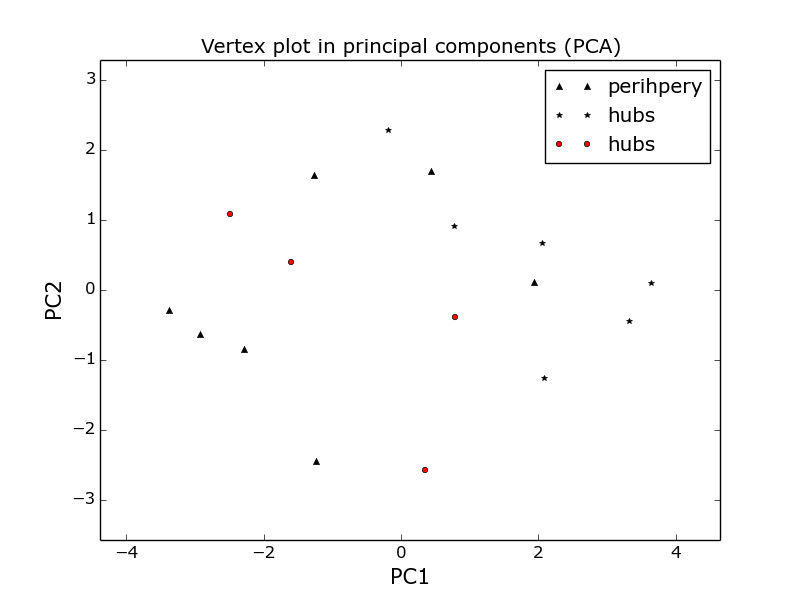
\includegraphics[width=0.3\textwidth]{figs/plot_pca}
	\caption{First two principal components.}
	\label{fig:formation}
\end{figure}



Principal components formation seem to be the less stable of all results reported in this study.
First component, with $\approx 25\%$ of dispersion, relies heavily on POS tags,
and slightly on sizes of tokens, sentences and messages.
Second component, with almost $12\%$ of dispersion, blends topology, POS tags and size of textual units.
Third component, with about $8.5\%$ of dispersion is mostly nouns frequency and size of textual units.
Fourth and fifth components present less than $5\%$ of total dispersion,
but are included in the Supporting Information document for completeness of exposition.

Tables~\ref{tab:pca1}-\ref{tab:pca5} yield these results and further insights.

\subsection{Results still to be interpreted}\label{subsec:sii}
%These networks yield diverse characteristics,
%some of which were not of core importance for this step of the research.
%Even so, at least one of these characteristics was found interesting enough to be considered a result and an example of interesting artifacts found.
Histogram differences of incident word sizes with and without repetition of words are constant.
That is, in each email list, when a histogram of word sizes were made with all words written,
and another histogram made with sizes of all \emph{different} words,
the cumulative absolute difference of the two histograms throughout the bins were found constant for all lists analysed.
When all known English words were considered, 
the difference sums up to $\approx 1.0$.
When stopwords are discarded,
the difference found was different, but still constant, slightly above $0.5$.
When only stopwords were considered, the difference is $\approx 0.6$.
When only known English words that does not have wordnet synsets are used,
this difference is $\approx 1.2$.
Appendix ~\ref{sec:resE} and Figures~\ref{fig:kw}-\ref{fig:nssnsw} are dedicated to this histogram differences.
% fazer plot desta diferença ao longo do aumento do número de mensagens (talvez de caracteres como metriac mais estável)
% Jogar td para o SI e só apontar este blueprint? TTM
%These results currently lacks substantial interpretation,
%which is provocative and should lead at least to a research note.

\section{Final remarks}\label{sec:remarks}
%Human interaction networks yield diverse linguistic peculiarities reported by its members.
This is a first systematic exploration of the relation between topological and textual
metrics in human interaction networks, as far the author knows.
Different textual features were scrutinized and were found to present
evident patterns, specially in relation to topological measures and the Erd\"os sectors.
%Results were regarded as stronger than envisioned from start, which poses diverse and intriguing questions.
%This results, confluent with recent research and development, some by the current author, are of core importance for social technologies and transformations, such as 
% Summarize main results TTM
Furthermore, results suggest that less connected participants bring external content and concepts,
while hubs qualify the content.
For example, periphery sectors present more nouns while hubs use more adjectives and usual words.
Such findings have potential applications in the collection and diffusion and information,
resources recommendation in linked data contexts, and open processes of document elaboration and refinement~\cite{ensaio,OPS,pnud5,evoSN,pbr}.

\subsection{Further work}\label{subsec:fw}

Similarity measures of texts in message-response threads has been thought about by the author, and some results are being organized.
These are two hypothesis obtained from recent experiments:
\begin{itemize}
    \item existence of information ``ducts'', observable through similarity measures. These might coincide with asymmetries of edges between vertexes pairs, with homophily or with message-response threads, to point just a few possibilities.
    \item Valuable insights can be derived from the self-similarity of messages by same author,
	    of messages sent at the same period of the day, etc.
	    This includes incidences of word sizes, incidences of tags and morphosintactic classes,
	    incidences of particular wordnet synset characteristics and wordnet word distances.
\end{itemize}

Current results suggests that diversity and self-similarity should vary with respect to connectivity. 
Literature usually assumes that periphery holds greater diversity~\cite{easley},
which can be further verified, for example through the diversity of entries.

Other potential next steps are:
\begin{itemize}
    \item The observation of most incident words and word types,
	    such as words related to cursing or to food.
    \item Interpretation of the results
	    exposed in Section~\ref{subsec:sii}.
    \item Extend word class observations, e.g. to include plurals, gender, common prefixes and suffixes.
    \item The observation of date and time in relation to textual production of interaction networks and
	    to activity characteristics (e.g. dispersion of sent time along the day or the week).
	    This was tackled by the author for the topological characterization of interaction networks~\cite{evoSN}, but left aside in this article.
	    % fazer aqui também ou em separado soh esse relacionamento TTM
    \item A careful analysis of each textual features distribution which is likely to reveal multimodal outlines and other non-trivial characteristics.
    \item Extend analysis to the windowed approach along the timelines used in the article where hub, peripheral and intermediary sectors where topologically characterized~\cite{evoSN}.
    \item For ELE list, the more connected the sector, the longer the messages are.
	    This is the inverse of what was found in the other lists,
	    and was considered a peculiarity of the culture bonded with the political subject of ELE list.
	    This hypothesis should be further verified.
    \item Tackle the same analysis on networks with languages other than English.
	    This is especially important for easing applications~\cite{ensaio}
	    and should rely on dedicated implementation of 
	    tokenization, lemmatization and attribution of POS tags.
    \item Observe a broader set of human interaction networks and the resulting types
	    of networks and participants with respect to topological and textual features.
    \item Analyse interaction networks from other platforms such as from LinkedIn and Facebook, etc.
    \item Sentiment analysis.
\end{itemize}


%\section{Acknowledgments}
%Renato Fabbri is grateful to CNPq 
%(processo 140860/2013-4, project 870336/1997-5);
%Postgraduate Committee of the IFSC/USP;
%%Prof. Dr. Leonardo Paulo Maia for the insights
%%which lead to the adaptation of the Kolmogorov-Smirnov
%%test presented in Appendix~\ref{sec:ks};
%GMANE
%developers and maintainers; participants of the
%mailing lists analysed.
%
\begin{acknowledgments}
	Financial support was obtained from CNPq (140860/2013-4,
	project 870336/1997-5), United Nations Development Program (contract: 2013/000566; project BRA/12/018) and FAPESP. 
	The authors are grateful to the GMANE creators and maintainers for the public email list data, to the communities of the email lists and other groups used in the analysis, and to the Brazilian Presidency of the Republic for keeping Participabr code and data open.
	We are also grateful to developers and users of Python scientific tools.
\end{acknowledgments}


%
% The following two commands are all you need in the
% initial runs of your .tex file to
% produce the bibliography for the citations in your paper.
\bibliographystyle{abbrv}
\bibliography{paper}  % sigproc.bib is the name of the Bibliography in this case
% You must have a proper ".bib" file
%  and remember to run:
% latex bibtex latex latex
% to resolve all references
%
% ACM needs 'a single self-contained file'!
%
%APPENDICES are optional
%\balancecolumns
%\newpage
\appendix
%\section{Support information}\label{sec:si}
%\subsection{Brief description of the email lists chosen}\label{subsec:gm}
%GMANE is a public email list database with some tenths of thousand of lists~\cite{GMANE}. Four email lists were selected, in a similar fashion developed in~\cite{evoSN}, but with MET substituted by ELE list so that all lists are in English. The lists are:
%\begin{itemize}
%    \item CPP, the development list of the standard C++ library\footnote{gmane.comp.gcc.libstdc++.devel is list ID in GMANE archive.}. Dominated by specialized computer programmers.
%    \item LAD: Linux Audio Developers list\footnote{gmane.linux.audio.devel is list ID in GMANE archive.}.
%    \item LAU: Linux Audio Users list\footnote{gmane.linux.audio.users is list ID in GMANE archive.}.
%    \item ELE: list for discussion of the election reform\footnote{gmane.politics.election-methods is list ID in GMANE}.
%\end{itemize}
%
%Table~\ref{tab:bas} has an overview of these lists, in terms of participants, threads and messages in each of the primitive connective sectors.

\section{Meaning of acronyms and abbreviations used the tables}
% completar tabela TTM
%\begin{table}[H]
%\centering
%\begin{tabular}{|p{1cm}|p{6cm}|}\hline
%symbol & meaning \\\hline\hline
%$|x|$ & the number of times $x$ was found \\\hline
%\emph{kw} & known word \\\hline
%$|x\neq|$ & number of different $x$ found \\\hline
%\emph{kwss} & known word with (wordnet) synset \\\hline
%\emph{kwsw} & known word that is a stopword \\\hline
%\emph{ukwsw} & unknown word that is a stopword \\\hline
%\emph{nsssw} & word without (wordnet) synset that is a stopword \\\hline
%\end{tabular}
%\end{table}

%Other symbols are explained on the tables itself.
Some concepts, such as \emph{contractions}, \emph{token} and \emph{char} are standard in natural language processing, and the reader is invited to visit~\cite{nltkBook}.
%\nocite{*}
\bibliography{paper}% Produces the bibliography via BibTeX.


%\balancecolumns
% That's all folks!
\end{document}

